\documentclass{article}
\usepackage{tikz}
\usepackage{gnuplot-lua-tikz}
\begin{document}
\begin{figure}
  \centering
  
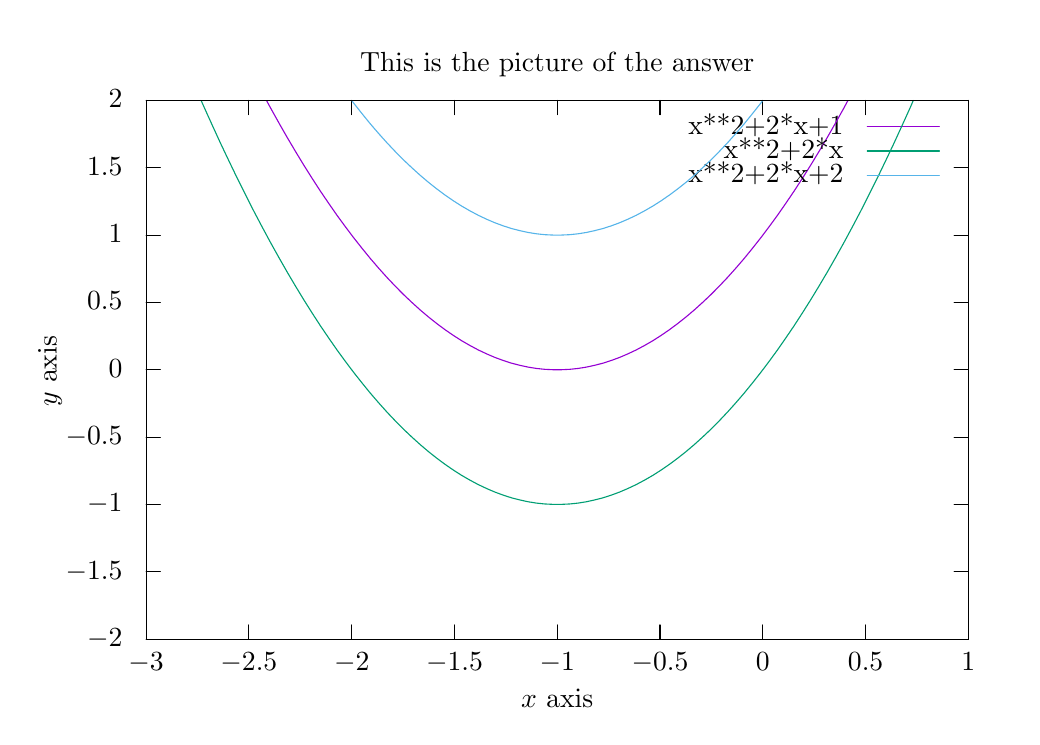
\begin{tikzpicture}[gnuplot]
%% generated with GNUPLOT 5.2p8 (Lua 5.3; terminal rev. Nov 2018, script rev. 108)
%% 2022年07月03日 星期日 23时12分39秒
\path (0.000,0.000) rectangle (12.500,8.750);
\gpcolor{color=gp lt color border}
\gpsetlinetype{gp lt border}
\gpsetdashtype{gp dt solid}
\gpsetlinewidth{1.00}
\draw[gp path] (1.504,0.985)--(1.684,0.985);
\draw[gp path] (11.947,0.985)--(11.767,0.985);
\node[gp node right] at (1.320,0.985) {$-2$};
\draw[gp path] (1.504,1.840)--(1.684,1.840);
\draw[gp path] (11.947,1.840)--(11.767,1.840);
\node[gp node right] at (1.320,1.840) {$-1.5$};
\draw[gp path] (1.504,2.695)--(1.684,2.695);
\draw[gp path] (11.947,2.695)--(11.767,2.695);
\node[gp node right] at (1.320,2.695) {$-1$};
\draw[gp path] (1.504,3.550)--(1.684,3.550);
\draw[gp path] (11.947,3.550)--(11.767,3.550);
\node[gp node right] at (1.320,3.550) {$-0.5$};
\draw[gp path] (1.504,4.405)--(1.684,4.405);
\draw[gp path] (11.947,4.405)--(11.767,4.405);
\node[gp node right] at (1.320,4.405) {$0$};
\draw[gp path] (1.504,5.260)--(1.684,5.260);
\draw[gp path] (11.947,5.260)--(11.767,5.260);
\node[gp node right] at (1.320,5.260) {$0.5$};
\draw[gp path] (1.504,6.115)--(1.684,6.115);
\draw[gp path] (11.947,6.115)--(11.767,6.115);
\node[gp node right] at (1.320,6.115) {$1$};
\draw[gp path] (1.504,6.970)--(1.684,6.970);
\draw[gp path] (11.947,6.970)--(11.767,6.970);
\node[gp node right] at (1.320,6.970) {$1.5$};
\draw[gp path] (1.504,7.825)--(1.684,7.825);
\draw[gp path] (11.947,7.825)--(11.767,7.825);
\node[gp node right] at (1.320,7.825) {$2$};
\draw[gp path] (1.504,0.985)--(1.504,1.165);
\draw[gp path] (1.504,7.825)--(1.504,7.645);
\node[gp node center] at (1.504,0.677) {$-3$};
\draw[gp path] (2.809,0.985)--(2.809,1.165);
\draw[gp path] (2.809,7.825)--(2.809,7.645);
\node[gp node center] at (2.809,0.677) {$-2.5$};
\draw[gp path] (4.115,0.985)--(4.115,1.165);
\draw[gp path] (4.115,7.825)--(4.115,7.645);
\node[gp node center] at (4.115,0.677) {$-2$};
\draw[gp path] (5.420,0.985)--(5.420,1.165);
\draw[gp path] (5.420,7.825)--(5.420,7.645);
\node[gp node center] at (5.420,0.677) {$-1.5$};
\draw[gp path] (6.726,0.985)--(6.726,1.165);
\draw[gp path] (6.726,7.825)--(6.726,7.645);
\node[gp node center] at (6.726,0.677) {$-1$};
\draw[gp path] (8.031,0.985)--(8.031,1.165);
\draw[gp path] (8.031,7.825)--(8.031,7.645);
\node[gp node center] at (8.031,0.677) {$-0.5$};
\draw[gp path] (9.336,0.985)--(9.336,1.165);
\draw[gp path] (9.336,7.825)--(9.336,7.645);
\node[gp node center] at (9.336,0.677) {$0$};
\draw[gp path] (10.642,0.985)--(10.642,1.165);
\draw[gp path] (10.642,7.825)--(10.642,7.645);
\node[gp node center] at (10.642,0.677) {$0.5$};
\draw[gp path] (11.947,0.985)--(11.947,1.165);
\draw[gp path] (11.947,7.825)--(11.947,7.645);
\node[gp node center] at (11.947,0.677) {$1$};
\draw[gp path] (1.504,7.825)--(1.504,0.985)--(11.947,0.985)--(11.947,7.825)--cycle;
\node[gp node center,rotate=-270] at (0.292,4.405) {$y$ axis};
\node[gp node center] at (6.725,0.215) {$x$ axis};
\node[gp node center] at (6.725,8.287) {This is the picture of the answer};
\node[gp node right] at (10.479,7.491) {x**2+2*x+1};
\gpcolor{rgb color={0.580,0.000,0.827}}
\draw[gp path] (10.663,7.491)--(11.579,7.491);
\draw[gp path] (3.033,7.825)--(3.086,7.728)--(3.192,7.538)--(3.297,7.354)--(3.403,7.175)%
  --(3.508,7.002)--(3.614,6.834)--(3.719,6.672)--(3.825,6.516)--(3.930,6.365)--(4.036,6.220)%
  --(4.141,6.081)--(4.247,5.947)--(4.352,5.818)--(4.458,5.695)--(4.563,5.578)--(4.669,5.466)%
  --(4.774,5.360)--(4.880,5.260)--(4.985,5.165)--(5.090,5.076)--(5.196,4.992)--(5.301,4.914)%
  --(5.407,4.841)--(5.512,4.774)--(5.618,4.713)--(5.723,4.657)--(5.829,4.607)--(5.934,4.562)%
  --(6.040,4.523)--(6.145,4.489)--(6.251,4.462)--(6.356,4.439)--(6.462,4.422)--(6.567,4.411)%
  --(6.673,4.406)--(6.778,4.406)--(6.884,4.411)--(6.989,4.422)--(7.095,4.439)--(7.200,4.462)%
  --(7.306,4.489)--(7.411,4.523)--(7.517,4.562)--(7.622,4.607)--(7.728,4.657)--(7.833,4.713)%
  --(7.939,4.774)--(8.044,4.841)--(8.150,4.914)--(8.255,4.992)--(8.361,5.076)--(8.466,5.165)%
  --(8.571,5.260)--(8.677,5.360)--(8.782,5.466)--(8.888,5.578)--(8.993,5.695)--(9.099,5.818)%
  --(9.204,5.947)--(9.310,6.081)--(9.415,6.220)--(9.521,6.365)--(9.626,6.516)--(9.732,6.672)%
  --(9.837,6.834)--(9.943,7.002)--(10.048,7.175)--(10.154,7.354)--(10.259,7.538)--(10.365,7.728)%
  --(10.417,7.825);
\gpcolor{color=gp lt color border}
\node[gp node right] at (10.479,7.183) {x**2+2*x};
\gpcolor{rgb color={0.000,0.620,0.451}}
\draw[gp path] (10.663,7.183)--(11.579,7.183);
\draw[gp path] (2.203,7.825)--(2.242,7.737)--(2.348,7.503)--(2.453,7.274)--(2.559,7.051)%
  --(2.664,6.833)--(2.770,6.621)--(2.875,6.414)--(2.981,6.213)--(3.086,6.018)--(3.192,5.828)%
  --(3.297,5.644)--(3.403,5.465)--(3.508,5.292)--(3.614,5.124)--(3.719,4.962)--(3.825,4.806)%
  --(3.930,4.655)--(4.036,4.510)--(4.141,4.371)--(4.247,4.237)--(4.352,4.108)--(4.458,3.985)%
  --(4.563,3.868)--(4.669,3.756)--(4.774,3.650)--(4.880,3.550)--(4.985,3.455)--(5.090,3.366)%
  --(5.196,3.282)--(5.301,3.204)--(5.407,3.131)--(5.512,3.064)--(5.618,3.003)--(5.723,2.947)%
  --(5.829,2.897)--(5.934,2.852)--(6.040,2.813)--(6.145,2.779)--(6.251,2.752)--(6.356,2.729)%
  --(6.462,2.712)--(6.567,2.701)--(6.673,2.696)--(6.778,2.696)--(6.884,2.701)--(6.989,2.712)%
  --(7.095,2.729)--(7.200,2.752)--(7.306,2.779)--(7.411,2.813)--(7.517,2.852)--(7.622,2.897)%
  --(7.728,2.947)--(7.833,3.003)--(7.939,3.064)--(8.044,3.131)--(8.150,3.204)--(8.255,3.282)%
  --(8.361,3.366)--(8.466,3.455)--(8.571,3.550)--(8.677,3.650)--(8.782,3.756)--(8.888,3.868)%
  --(8.993,3.985)--(9.099,4.108)--(9.204,4.237)--(9.310,4.371)--(9.415,4.510)--(9.521,4.655)%
  --(9.626,4.806)--(9.732,4.962)--(9.837,5.124)--(9.943,5.292)--(10.048,5.465)--(10.154,5.644)%
  --(10.259,5.828)--(10.365,6.018)--(10.470,6.213)--(10.576,6.414)--(10.681,6.621)--(10.787,6.833)%
  --(10.892,7.051)--(10.998,7.274)--(11.103,7.503)--(11.209,7.737)--(11.247,7.825);
\gpcolor{color=gp lt color border}
\node[gp node right] at (10.479,6.875) {x**2+2*x+2};
\gpcolor{rgb color={0.337,0.706,0.914}}
\draw[gp path] (10.663,6.875)--(11.579,6.875);
\draw[gp path] (4.115,7.825)--(4.141,7.791)--(4.247,7.657)--(4.352,7.528)--(4.458,7.405)%
  --(4.563,7.288)--(4.669,7.176)--(4.774,7.070)--(4.880,6.970)--(4.985,6.875)--(5.090,6.786)%
  --(5.196,6.702)--(5.301,6.624)--(5.407,6.551)--(5.512,6.484)--(5.618,6.423)--(5.723,6.367)%
  --(5.829,6.317)--(5.934,6.272)--(6.040,6.233)--(6.145,6.199)--(6.251,6.172)--(6.356,6.149)%
  --(6.462,6.132)--(6.567,6.121)--(6.673,6.116)--(6.778,6.116)--(6.884,6.121)--(6.989,6.132)%
  --(7.095,6.149)--(7.200,6.172)--(7.306,6.199)--(7.411,6.233)--(7.517,6.272)--(7.622,6.317)%
  --(7.728,6.367)--(7.833,6.423)--(7.939,6.484)--(8.044,6.551)--(8.150,6.624)--(8.255,6.702)%
  --(8.361,6.786)--(8.466,6.875)--(8.571,6.970)--(8.677,7.070)--(8.782,7.176)--(8.888,7.288)%
  --(8.993,7.405)--(9.099,7.528)--(9.204,7.657)--(9.310,7.791)--(9.335,7.825);
\gpcolor{color=gp lt color border}
\draw[gp path] (1.504,7.825)--(1.504,0.985)--(11.947,0.985)--(11.947,7.825)--cycle;
%% coordinates of the plot area
\gpdefrectangularnode{gp plot 1}{\pgfpoint{1.504cm}{0.985cm}}{\pgfpoint{11.947cm}{7.825cm}}
%\draw[gp path] (-3,0) -- (1,0);
%\draw (0,-2) -- (0,2);
\end{tikzpicture}
%% gnuplot variables

\caption{The picture of the answer}

\end{figure}
\end{document}
